\documentclass[11pt, oneside]{article}   	% use "amsart" instead of "article" for AMSLaTeX format
\usepackage{geometry}              		% See geometry.pdf to learn the layout options. There are lots.
\usepackage{amsmath}
\geometry{letterpaper}                   		% ... or a4paper or a5paper or ... 
%\geometry{landscape}                		% Activate for rotated page geometry
%\usepackage[parfill]{parskip}    		% Activate to begin paragraphs with an empty line rather than an indent
\usepackage{graphicx}				% Use pdf, png, jpg, or eps§ with pdflatex; use eps in DVI mode
								% TeX will automatically convert eps --> pdf in pdflatex		
\usepackage{amssymb}

%SetFonts

%SetFonts


\title{Homework 1}
\author{Weiyu Yan}
\date{}							% Activate to display a given date or no date

\begin{document}
\maketitle
\section{Perceptron Algorithm and Convergence Analysis}

\begin{enumerate}
\item	%1
  \begin{enumerate}
  \item	%a
    $ y=f(x_1,x_2)=x_1 $\\
    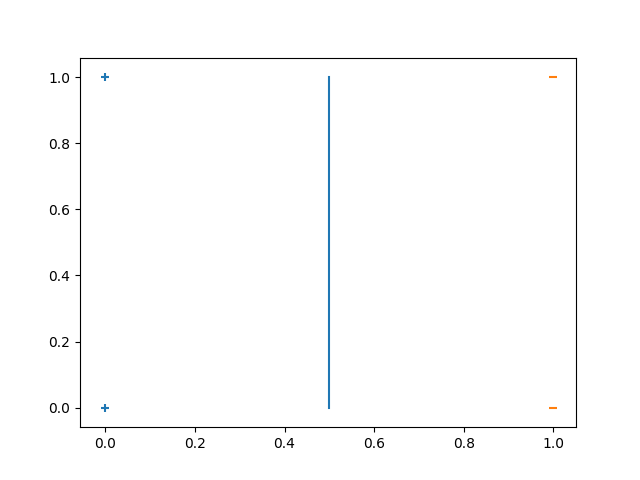
\includegraphics[width=15cm]{1.1a.png}\\
  \item	%b
    A truth table for this function could be:\\
    \begin{tabular}{|c|c|c|}
      \hline
      $x_1$ & $x_2$ & $y$ \\ \hline
      0     & 0     & 1   \\ \hline
      0     & 1     & 0   \\ \hline
      1     & 0     & 0   \\ \hline
      1     & 1     & 1   \\ \hline
    \end{tabular}\\
    We can plot those points in a figure.\\
    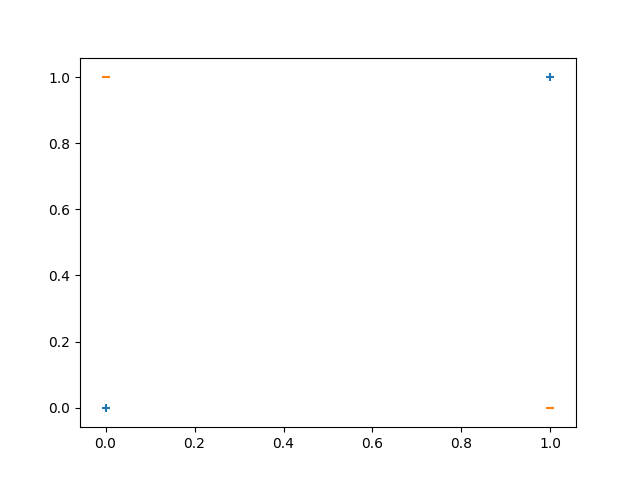
\includegraphics[width=15cm]{1.1b.png}
    The perceptron algorithm gives us a weight vector which corresponds to its orthogonal hyperplane to divide points into 2 parts. In this figure since we can't find a hyperplane to divide the 2 kinds, this function can't be separated by single perceptron.
  \item	%c
    $ y=f(x_1,x_2,x_3)=x_3 $\\
    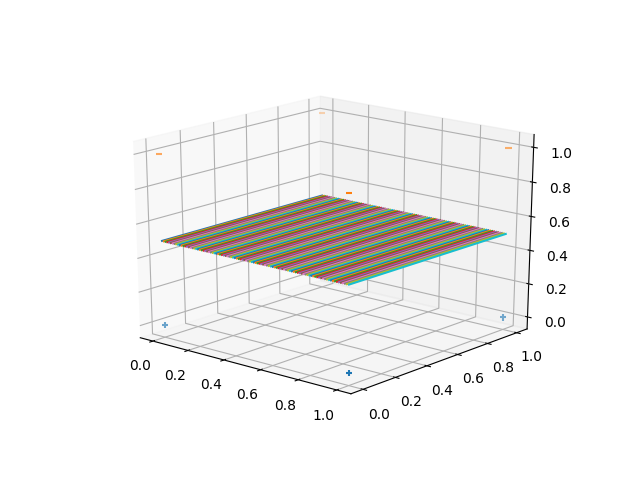
\includegraphics[width=15cm]{1.1c.png}\\
  \end{enumerate}

\item %2
  $\beta$ is a weight vector perpendicular to the hyperplane
  the signed Euclidean Distance of the point $x$ to the hyperplane is given by:
  \[
  d=\frac{(x-x_0) \cdot \beta y} {\left \| \beta \right \|_2}\\
  \]
  where
  \[
  x_0 \in \{x|f(x)=0\}
  \]
  \[
  \because f(x_0)=\beta_0 + \beta^Tx_0
  \]
  \[
  \therefore \beta^T x_0 = -\beta_0
  \]
  Therefore
  \begin{equation}
    \begin{split}
      d&=\frac{y(x \cdot \beta - x_0 \cdot \beta)} {\left \| \beta \right \|_2}\\
      &=\frac{y(\beta^T x - \beta^T x_0)} {\left \| \beta \right \|_2}\\
      &=\frac{y(\beta^T x + \beta_0)} {\left \| \beta \right \|_2}\\
      &=\frac{yf(x)} {\left \| \beta \right \|_2}
    \end{split}
  \end{equation}

\item
  By perceptron convergence theorem we get that the perceptron algorithm makes at most $\frac{1}{\delta^2}$ mistakes where $\frac{1}{\delta^2}$ is the lower bound for $y_i(w^{sep^T}x_i)$ and $w^{sep}$ is the ``good separator'':
  \[
  T \leq \frac{1}{\delta^2}
  \]
  where
  \[
  y_i(w^{sep} x_i) \geq \delta
  \]
  Since
  \[
  y_i w^{sep} x_i =1
  \]
  we have
  \[
  T \leq 1
  \]
  Since $w^{0}=0$, $\|w^{sep}\|=1$, we have:
  \[
  \| w^{(0)} - w^{sep} \|^2_2 = \| w^{sep} \|^2_2 = 1
  \]
  Therefore,
  \[
  T \leq \| w^{(0)} - w^{sep} \|^2_2
  \]  
 % Since $w^t$ converges to $w^{sep}$ after $T$ steps, we have:
 % \[
 % \| w^{(0)} - w^{sep} \|^2_2 = 
  % \]
%  \because \|w^{sep}\|_2=1\\
%\therefore \| w^{(0)} - w^{sep} \|_2 = \| w^{(0)} - w^{sep} \|_2 \| w^{sep}\|_2\\
% \geq \| w^{sep} (w^{(0)} - w^{sep}) \|_2 \\
%= \| w^{sep} \sum_{t=1}^{T} (w^{t-1}-w^{t}) \|^2_2
%= \| w^{sep} \sum_{t=1}^{T} (w^{t-1}-w^{t}) \|^2_2
%= \| w^{sep} \sum_{t=1}^{T} y_i x_i \|^2_2
%= \| \sum_{t=1}^{T} w^{sep}y_i x_i \|^2_2
%=|-T|
%=T
%= \sum_{1}^{T} \| y_i x_i \|^2_2
\end{enumerate}


\section{Programming Assignment}

\begin{enumerate}
\item	%1
  Please refer code in "perceptron.py"
  \begin{enumerate}
  \item	%a
    Epoch number is set to 100. The figure is shown below:\\
    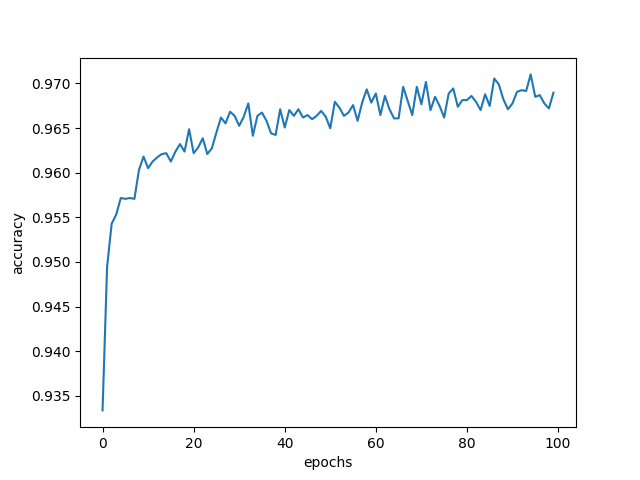
\includegraphics[width=15cm]{2.1a.png}\\
    The accuracy increases drastically before $ I \approx 15 $. Then it rises shakingly and slowly.\\
    By increasing/decreasing $ I $ the shape of the curve won't change but just reveals more/less of the curve in the figure.
    
  \item	%b
    Epoch number is set to 100. The figure is shown below:\\
    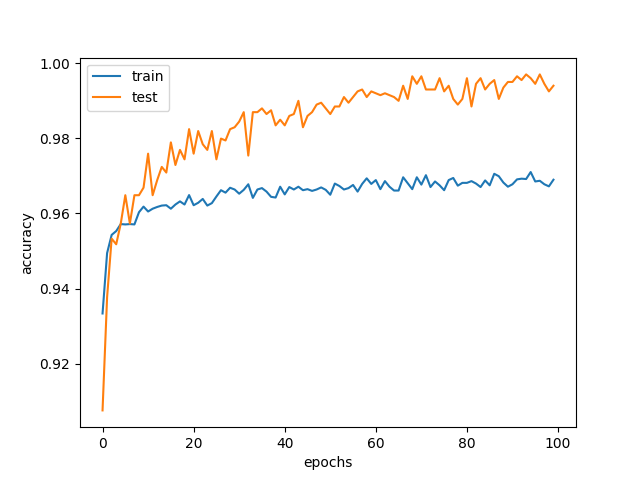
\includegraphics[width=15cm]{2.1b.png}\\
    Red one is for training data, while blue one is for testing data.\\
    For testing data, the result is even better. As the accuracy continues to rise(shakingly).
  \item	%c
    accuracy:  0.9939728779507785\\
    confusion matrix:
    \[
    \left[
      \begin{array}{cc}
	1009	&	40\\
	0	&	942
      \end{array}
      \right]
    \]
  \item %d
    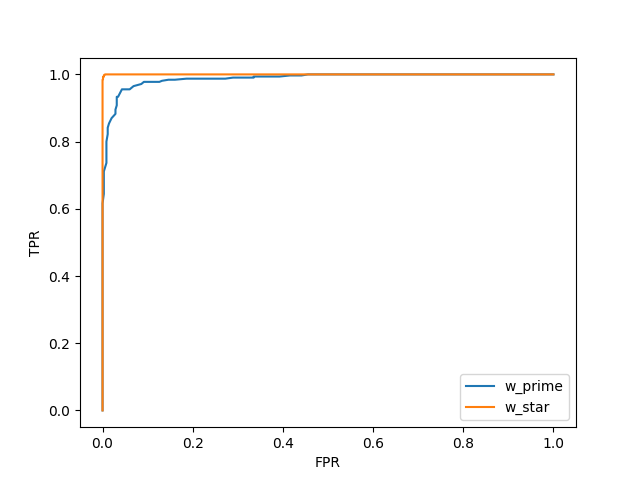
\includegraphics[width=15cm]{2.1d.png}
  \item %e
    AUC($ w^\prime) = 0.9877518533678995$\\
    AUC($ w^*) = 0.9999666948582919$
    The greater the AUC value, the bigger area that is under the ROC curve, the 'upper' that the ROC curve goes.
  \end{enumerate}

\item %2
  \begin{enumerate}
  \item
    
  \item
    
  \end{enumerate}
\end{enumerate}






\end{document}  
